%; whizzy paragraph -pdf xpdf -latex ./whizzypdfptex.sh
%; whizzy-paragraph "^\\\\begin{frame}\\|\\\\emtext"
% latex beamer presentation.
% platex, latex-beamer でコンパイルすることを想定。 

%     Tokyo Debian Meeting resources
%     Copyright (C) 2012 Junichi Uekawa

%     This program is free software; you can redistribute it and/or modify
%     it under the terms of the GNU General Public License as published by
%     the Free Software Foundation; either version 2 of the License, or
%     (at your option) any later version.

%     This program is distributed in the hope that it will be useful,
%     but WITHOUT ANY WARRANTY; without even the implied warreanty of
%     MERCHANTABILITY or FITNESS FOR A PARTICULAR PURPOSE.  See the
%     GNU General Public License for more details.

%     You should have received a copy of the GNU General Public License
%     along with this program; if not, write to the Free Software
%     Foundation, Inc., 51 Franklin St, Fifth Floor, Boston, MA  02110-1301 USA

\documentclass[cjk,dvipdfmx,12pt]{beamer}
\usetheme{Tokyo}
\usepackage{monthlypresentation}

%  preview (shell-command (concat "evince " (replace-regexp-in-string "tex$" "pdf"(buffer-file-name)) "&")) 
%  presentation (shell-command (concat "xpdf -fullscreen " (replace-regexp-in-string "tex$" "pdf"(buffer-file-name)) "&"))
%  presentation (shell-command (concat "evince " (replace-regexp-in-string "tex$" "pdf"(buffer-file-name)) "&"))

%http://www.naney.org/diki/dk/hyperref.html
%日本語EUC系環境の時
\AtBeginDvi{\special{pdf:tounicode EUC-UCS2}}
%シフトJIS系環境の時
%\AtBeginDvi{\special{pdf:tounicode 90ms-RKSJ-UCS2}}

\newenvironment{commandlinesmall}%
{\VerbatimEnvironment
  \begin{Sbox}\begin{minipage}{1.0\hsize}\begin{fontsize}{8}{8} \begin{BVerbatim}}%
{\end{BVerbatim}\end{fontsize}\end{minipage}\end{Sbox}
  \setlength{\fboxsep}{8pt}
% start on a new paragraph

\vspace{6pt}% skip before
\fcolorbox{dancerdarkblue}{dancerlightblue}{\TheSbox}

\vspace{6pt}% skip after
}
%end of commandlinesmall

\title{東京エリアDebian勉強会 x 関東LibreOfficeオフ}
\subtitle{第119回 2014年10月度2nd}
\author{野島貴英}
\date{2014年10月25日}
\logo{
\includegraphics[width=8cm]{image200607/openlogo-light.eps}}

\begin{document}

\begin{frame}
\titlepage{}
\end{frame}

\begin{frame}{設営準備にご協力ください。}
会場設営よろしくおねがいします。
\end{frame}

\begin{frame}{Agenda}
 \begin{minipage}[t]{0.45\hsize}
  \begin{itemize}
   \item 注意事項
	 \begin{itemize}
	  \item 写真はセミナールーム内のみ可です。
          \item 出入りは自由でないので、もし外出したい方は、野島まで一声くださいませ。
	 \end{itemize}
   \item 事前課題発表
  \end{itemize}
 \end{minipage} 
 \begin{minipage}[t]{0.45\hsize}
  \begin{itemize}
   \item 最近あったDebian関連のイベント報告
	 \begin{itemize}
	  \item 第117回 東京エリアDebian勉強会
	  \item 第118回 東京エリアDebian勉強会 in OSC tokyo/fall
	 \end{itemize}
   \item Debian Trivia Quiz
   \item DebConf14のビデオ紹介
   \item 今後のイベント
   \item 今日の宴会場所
  \end{itemize}
 \end{minipage}
\end{frame}

\section{事前課題}
\emtext{事前課題}
{\footnotesize
\begin{prework}{ 野島 貴英 }
もちろん!Jessieインストーラテスト会に参加します。
よろしくお願いします。
\end{prework}

\begin{prework}{ henrich }
フリーズ前の課題洗い出しとか…。
\end{prework}

\begin{prework}{ dictoss(杉本 典充) }
Jessieインストーラテスト会に参加します。
\end{prework}

\begin{prework}{ 吉野(yy\_{}y\_{}ja\_{}jp) }
DDTSS
\end{prework}

\begin{prework}{ kenhys }
groonga-normalizer-mysqlのITP関連
\end{prework}

\begin{prework}{ Hasegawa }
Jessieインストーラテスト会に参加します。
よろしくお願いします。
\end{prework}

}

\section{イベント報告}
\emtext{イベント報告}

\begin{frame}{第117回東京エリアDebian勉強会}
 
\begin{itemize}
\item 場所はスクウェア・エニックスさんのセミナルームをお借りしての開催でした。6名の参加がありました。
\begin{itemize}
\item 野島さんにてDebConf14のビデオのトピックについて、
\item やまねさんにより、DebConf14の様子について口頭にて、
\end{itemize}
発表が行われました。
\item 残りの時間はもくもく会を行い、最後に成果発表をしました。
\item 今回は宴会の参加者が居なかったため、代わりに3名で夕食会となりました。
\end{itemize} 
\end{frame}

\begin{frame}{第117回東京エリアDebian勉強会(続き)}

 DebConf14では日本側からの発表が2本あったのは大変すばらしいと思います。
また、DebConf14のzackさんの発表「Debian in the Dark Ages of Free Software」は、Debian開発関係者には
非常に困った事態だと思います。こちらについては今後も真剣に考えていきたいと思います。

\end{frame}

\begin{frame}{第118回東京エリアDebian勉強会 in OSC 2014 Tokyo/Fall}

 OSC 2014 tokyo/fallへ東京エリアDebian勉強会として出張しました。 

\begin{itemize}
\item 10/18(土)にて岩松さんによりセミナ開催、Debianについてのブース出しを行いました。また、Debian Officail DeveloperのPaulLiuさんが遥々台湾から参加されました。
\item 10/19(日)は元々計画していませんでしたが、koedoyoshidaさんの厚意により、ブースを出していただきました。
\end{itemize} 
 
 10/18(土)のOSC 2014 tokyo/fallの参加者が、900名を超えたそうです。こういったイベントで盛り上げることにより、FOSS関係者やコミュニティが益々増えると良いですね。
 
\end{frame}


\section{Debian Trivia Quiz}
\emtext{Debian Trivia Quiz}
\begin{frame}{Debian Trivia Quiz}

  Debian の常識、もちろん知ってますよね?
知らないなんて恥ずかしくて、知らないとは言えないあんなことやこんなこと、
みんなで確認してみましょう。

今回の出題範囲は\url{debian-devel-announce@lists.debian.org},
\url{debian-news@lists.debian.org} に投稿された
内容などからです。

\end{frame}

\subsection{問題}

%; whizzy-master ../debianmeetingresume201311.tex
% 以上の設定をしているため、このファイルで M-x whizzytex すると、whizzytexが利用できます。
%

\santaku
{2014/9/14時点でJessieでサポートされると残念ながら「言われなかった」アーキテクチャはどれ}
{amd64}
{powerpc}
{sparc}
{C}
{2014/9/14時点でサポートされると言われたアーキテクチャは:amd64,armel,armhf,i386,kfreebsd-amd64/kfreebsd-i386/mips/mipsel/powerpc/s390x。なお、arm64/ppc64elは好調な頑張りとのことで、この調子が続けば入るかも??という状況。}

\santaku
{2014/11/1時点でJessieでサポートされるかどうかについて依然として懸念のあるものはどれ}
{hurd}
{kFreeBSD}
{s390x}
{B}
{kFreeBSDは頑張って欲しいとのこと。最終ジャッジは2014/11/1に行われる。なお、s390xは9/14では懸念なし、hurdはすでにリリースは無理との判断になっている。}

\santaku
{2014/9/4にtesting入りしたデスクトップ環境は以下のどれ}
{xfce}
{cinnamon}
{unity}
{B}
{cinnamonはGTK+3を利用して作られたデスクトップ環境です。元々はLinux MINT向けにGNOME Shellからforkしたデスクトップシェルでした。開発が続き、デスクトップシェルから発展して遂にデスクトップ環境となりました。}

\santaku
{2014/10/18にリリースされたwheezyのDebianのバージョンはいくら?}
{7.7}
{7.8}
{7.9}
{A}
{7回目のアップデートとなります。早速アップグレードしましょう!新規にインストールする安定版ならDebian7.7からやりましょう!}

\santaku
{OPWの呼びかけがdebian-devel-announceで2014/9/30に行われました。ところでOPWって何の略?}
{One-time PassWord}
{One-Piece-Woven technology}
{Outreach-Program-for-Women}
{C}
{Outreach-Program-for-Women(略してOPW)は、GNOME Foundationが始めた、FOSSのプロジェクトの貢献者にもっと女性を増やそう!という活動となります。FOSSの貢献者の男女構成比は、圧倒的に男の割合が高いといういびつな傾向があるため、こちらを是正しようとする活動です。}

\santaku
{2014/10/14にサービスを近いうちに閉じるよとアナウンスのあったサイトはどれでしょう?}
{githubredir.debian.net}
{tracker.debian.org}
{rtc.debian.org}
{A}
{githubredir.debian.netは、github上にあるupstreamのソースについて、リリースの為にバージョン番号でtag打ちされたバージョンのソースのtarボールに対する直接のリンクを統一的な書式のURLで生成するサービスです。つまり、debian/watchにupstreamのソースの有りかを書きやすくするために使われます。githubが改善され今となっては不要となってしまったということもあり、近いうちに廃止するというアナウンスが行われました。}

\santaku
{2014/10/5にリリースされたDebian Installer Jessie Beta2の変更点はどれ}
{syslinuxまわりで過去の互換の無い大きな変更点が出た。}
{デフォルトのinitがsystemdとなった。}
{GNOMEデスクトップ環境がデフォルトになった。}
{C}
{一度はXfceデスクトップ環境と言われていましたが、accessibilityの完成度の高さには勝てず、再びGNOMEに戻ってきた形となりました。なお、他の選択肢はBeta1の時の変更点となります。}

\santaku
{2014/10/16に投票が開始されました。内容は次のうちどれ?}
{特定のinitとプログラムが依存しても良いか?ダメか?程度次第か?}
{GNOMEをデフォルトにしてよいのか?}
{野島が勉強会幹事をやり続けて良いのか?}
{A}
{Debianの各種initシステムと他アプリケーションの依存についての規定に関する投票となります。投票内容について詳しくはhttps://www.debian.org/vote/2014/vote\_003。ところで、Debianのイベントの幹事は、もちろん、いつ、誰が、どのようにやってもよくてよ?勇者の数を増やせ!}


\section{Debian x LibreOffice}
\emtext{Debian x LibreOffice}

\begin{frame}{ようこそ}

 祝!関東LibreOfficeオフさんと共同で勉強会開催!

\end{frame}

\begin{frame}{Debianとupstreamの関係の方針}

\center{\Large 一言で言えば Win-Winになりましょう!}

\begin{itemize}
\item 基本upstream firstです。
\item 理想は、Debian固有のパッチだけでパッケージを作り、そうじゃないパッチはできるだけupstreamへフィードバックします。
\item upstreamとの連携は重要です。FOSS界でディストリビューションを通して利用者のHubになることを目指しています。
\end{itemize}

\end{frame}

\begin{frame}{Debianとupstreamの関係の方針}

\begin{figure}[H]
\begin{center}
 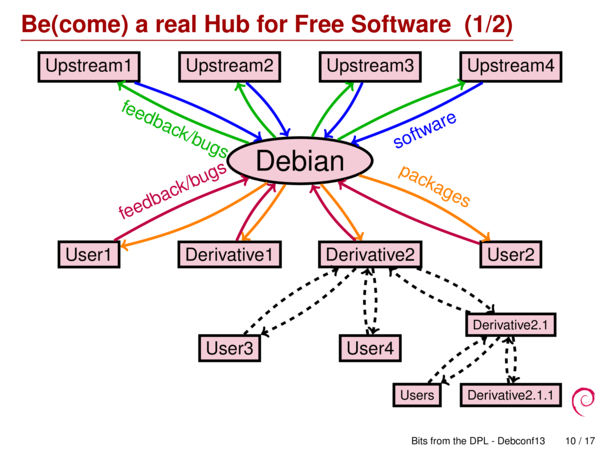
\includegraphics[width=0.7\hsize]{image201410/debian-hub.png}
\end{center}
\caption{DPLの2013のプレゼンから抜粋}
\end{figure}

\url{http://www.lucas-nussbaum.net/blog/wp-content/uploads/2013/08/bits.pdf}

\end{frame}

\begin{frame}{DebianとLibreOfficeのバージョン}

\begin{table}[ht]
\begin{center}
\small
\begin{tabular}{|l|p{3cm}|l|l|}
\hline 
Debian&Debianアーキテクチャ&LibreOfficeバージョン& 備考\\ \hline \hline
wheezy(stable) & amd64 armel armhf i386 ia64 kfreebsd-amd64 kfreebsd-i386 mips mipsel powerpc s390 s390x sparc & 3.5.4 & \\ \hline
jessie(testing) & amd64 arm64 armel armhf i386 kfreebsd-amd64 kfreebsd-i386 mips mipsel powerpc ppc64el s390x & 4.3.2 & \\ \hline
\end{tabular}
\end{center}
\end{table}

\end{frame}

\begin{frame}{DebianとLibreOfficeのバージョン}

\begin{table}[ht]
\begin{center}
\small
\begin{tabular}{|l|p{3cm}|l|l|}
\hline 
Debian&Debianアーキテクチャ&LibreOfficeバージョン& 備考\\ \hline \hline
sid(unstable) & amd64 armel armhf i386 kfreebsd-amd64 kfreebsd-i386 mipsel powerpc ppc64el s390x sparc & 4.3.3 & \\ \cline{2-4} 
 & arm64 mips alpha ppc64 & 4.3.2 & \\ \hline
experimental & amd64 armhf i386 ppc64el & 4.4.0 & \\ \hline
\end{tabular}
\end{center}
\end{table}
\end{frame}

\begin{frame}{使う側のDebian固有の事情の情報源}

\begin{table}[ht]
\begin{center}
\small
\begin{tabular}{|l|p{7cm}|}
\hline
種別 & 場所  \\ \hline \hline
ファイル & /usr/share/doc/libreoffice/README.Debian  \\ \hline
wiki & \url{https://wiki.debian.org/LibreOffice}  \\ \hline
bugレポート & \url{https://bugs.debian.org/libreoffice}  \\ \hline
\end{tabular}
\end{center}
\caption{Debian固有のLibreOffice情報}
\label{tab:debian-specific-about-libreoffice}
\end{table}


\end{frame}

\begin{frame}{メンテナ(理想)}

 DebianでのLibreOfficeのパッケージ開発は、Debian LibreOffice Maintainers ( debian-openoffice\@lists.debian.org )という
コミュニティが用意されています。

\end{frame}

\begin{frame}{メンテナ(現実)}

 DebianについてはRene Engelhardさんにより精力的にメンテナンスが行われている状態です。
 
\end{frame}

\begin{frame}{パッケージのソースコード}

 Debianのパッケージの開発のgitリポジトリは、\url{http://anonscm.debian.org/cgit/pkg-openoffice/libreoffice.git}で管理されています。各ブランチが切られており、ubuntu用なども見えます。

\end{frame}

\begin{frame}{パッケージのソースコード}

 また、apt-get source libreofficeすると、debian/README.debian-sourceが入っています。こちらを読むと判りますが、

\begin{itemize}
\item バージョンアップしたパッケージをどう作るかについて、工数が少なくなるような、一定のやり方を定めています。debian/rulesファイルも、非常にうまく作られていて、このやり方で多くの事が出来るようになっています。
\item LibreOffice自体巨大なソースですので、必然的にdebian/controlファイルも巨大化します。こちらをメンテしやすくするため、パッケージの種別毎にcontorlファイルが多数分割されており、debian/rulesでcontrolファイルを生成できるようになっています。
\end{itemize}

\end{frame}

\begin{frame}{パッケージのソースコード}

\begin{itemize}
\item debian/*.inファイルを使って、パッケージ内部に梱包する様々な設定ファイルを各Debianの環境に合わせて修正・合成しています。
\item dpkg-devで梱包されている/usr/share/dpkg/*.mkファイルに基づき、configureに必要なオプションが作られていきます。
\item DFSG Freeにこだわる必要があるため、openoffice由来のソースから、DFSG Freeでないものを抹消しています。
\end{itemize}

\end{frame}

\begin{frame}{Debian固有のパッチの紹介}

 いくつもパッチがありますが、Debian固有で面白いものを抜き出して列挙してみます。

 \begin{itemize}
  \item aarch64.diff \\
    arm64用のパッチ。unoを取うためのarm64用のコードが追加されている。
  \item aotcompile-256M-default.diff \\
    MAX\_CLASSES\_PER\_JAR = 256,MAX\_BYTES\_PER\_JAR = 262144をビルドマシンの搭載メモリサイズによらず固定にするパッチ。
 \end{itemize}

\end{frame}

\begin{frame}{Debian固有のパッチの紹介}

 \begin{itemize}
  \item config-sub-guess-update.diff \\
    システムがglibc/ulibc/dietlibcであるかを検出して適切なLIBC変数を設定する。さらに、古いシステム(Next、hp300、386BSD等...)の判定コードを削除。(他もやっているがDebianシステムに関わる部分だけ記載)
  \item debian-hardened-buildflags-CPPFLAGS.diff \\ 
    Jessieリリースゴールの1つであるhardeningを搭載する。
  \item sensible-lomua.diff,help-msg-add-package-info.diff,reportdesign-mention-package.diff,jurt-soffice-location.diff \\
    Debianの環境でMUAをどれにする、ヘルプファイルのパッケージ導入を促す、report-builderのパッケージ導入を促す,sofficeのPATHを返す。
  \item system-coinmp.diff \\
   coinmpに対応する。
 \end{itemize}

\end{frame}

\begin{frame}{Debian固有のパッチの紹介}

 \begin{itemize}
  \item split-evoab.diff \\
    gnomeのMUAであるevolutionのアドレス帳連携のドライバでEVOAB2を有効にするパッチ。
  \item earch-usr-share-for-images.diff \\
    画像のサーチパスの検索順番をdebianにあわせるべく変更(プログラムの改造含む)。
  \item debian-debug.diff \\
    -g1をgccのデバッグオプションとして利用し、デバッグシンボルファイルのサイズを減らす。
  \item gcj-safe-jni-h-include.diff \\
    gcjで、jni.hがシステムにあわせてincludeされるように変更。
 \end{itemize}

\end{frame}

\begin{frame}{いくつか用語説明}

 \begin{itemize}
 \item uno\\
 Universal Network Object。CORBAとかCOM(DCOM)等のオブジェクト指向の通信により、LibreOfficeのAPI呼び出しを実現する仕組み。
 \url{https://wiki.openoffice.org/wiki/Documentation/DevGuide/ ProUNO/Introduction}
 \item hardening\\
 コンパイラにセキュリティ強化の施策を打たせる事。\url{https://wiki.debian.org/Hardening}
 \item coinmp \\
  COmputational Infrastructire for Operations Research(CON-OR)のライブラリ。OR用途。\url{https://projects.coin-or.org/}
 \end{itemize}
\end{frame}

\begin{frame}[containsverbatim]{LibreOffice 4.3を使う}

 以下は簡易版なやり方(本来はtestingからアップグレードが望ましい)
 \begin{description}
 \item [Step1.]  Debian安定版を導入。
 \item [Step2.]  /etc/apt/source.listを内容を全部以下に置き換え。
 \end{description}

 \begin{commandlinesmall}
deb http://ftp.jp.debian.org/debian/ sid main contrib non-free
deb-src http://ftp.jp.debian.org/debian/ sid main contrib non-free
 \end{commandlinesmall}

\end{frame}

\begin{frame}{LibreOffice 4.3を使う}

 \begin{description}
 \item [Step3.]  aptitude update; aptitude full-upgradeする。
 \item [Step4.]  aptitude install systemd を実行。
  \item [Step5.]  aptitude install libreoffice/sid を実行。
  \item [Step6.]  hash; libreoffice を実行。
 \end{description}
\end{frame}

\begin{frame}[containsverbatim]{LibreOffice 4.4を使う}

 続けて\\
    Step7. /etc/apt/source.listを内容を全部以下を追記

 \begin{commandlinesmall}
deb http://ftp.jp.debian.org/debian/ experimental main contrib non-free
deb-src http://ftp.jp.debian.org/debian/ experimental main contrib non-free
 \end{commandlinesmall}

\end{frame}

\begin{frame}{LibreOffice 4.4を使う}

 \begin{description}
 \item [Step 8.]  aptitude update する。
  \item [Step 9.]  aptitude -t experimental install libreoffice
  \item [Step 10.]  hash; libreoffice を実行。
 \end{description}
\end{frame}

\begin{frame}{おわりに}

 最新版を是非使っていただきまして、

 \begin{center}
\LARGE 是非、バグレポ書こう!パッチ書こう!
 \end{center}

\end{frame}

\section{今後のイベント}
\emtext{今後のイベント}
\begin{frame}{今後のイベント}
\begin{itemize}
 \item 関西エリアDebian勉強会
 \item 東京エリアDebian勉強会 
\end{itemize}
\end{frame}

\section{今日の宴会場所}
\emtext{今日の宴会場所}
\begin{frame}{今日の宴会場所}
未定
\end{frame}

\end{document}

;;; Local Variables: ***
;;; outline-regexp: "\\([ 	]*\\\\\\(documentstyle\\|documentclass\\|emtext\\|section\\|begin{frame}\\)\\*?[ 	]*[[{]\\|[]+\\)" ***
;;; End: ***
